\documentclass[10pt, conference, compsocconf, a4paper]{IEEEtran}
%\usepackage{CJKutf8}
\usepackage[UTF8]{ctex}
\usepackage{cite}
\usepackage{amsmath,amssymb,amsfonts}
%\usepackage{algorithmic}
\usepackage{graphicx}
\usepackage{textcomp}
%\usepackage{pythonhighlight}
\usepackage{enumerate}
\usepackage{verbatim}
\hyphenation{op-tical net-works semi-conduc-tor}

% 中英文摘要并存
\newcommand{\enabstractname}{Abstract}
\newenvironment{enabstract}{%
    \par\small
    \noindent\mbox{}\hfill{\bfseries \enabstractname}\hfill\mbox{}\par
    \vskip 2.5ex}{\par\vskip 2.5ex}  



\begin{document}
	%\begin{CJK}{UTF8}{gbsn}

\title{基本共射极放大电路的仿真与探究}

\author{
  薛昊辰,于宗玄,高浚哲,麻柯柯,胡潇丹
}

% 选择作者样式
\begin{comment}
\author{
  \IEEEauthorblockN{薛昊辰}
  \IEEEauthorblockA{
    西安邮电大学\\
    03185002
  }
  \and
  \IEEEauthorblockN{于宗玄}
  \IEEEauthorblockA{
    西安邮电大学\\
    03185002
  }
  \and
  \IEEEauthorblockN{高浚哲}
  \IEEEauthorblockA{
    西安邮电大学\\
    03185002
  }
  \and
  \IEEEauthorblockN{麻柯柯}
  \IEEEauthorblockA{
    西安邮电大学\\
    03185002
  }
  \and
  \IEEEauthorblockN{胡潇丹}
  \IEEEauthorblockA{
    西安邮电大学\\
    03185002
  }
}
\end{comment}


\maketitle


% TODO: 修改摘要

% 中文摘要
%\begin{abstract}
%本文详述了基本共射极放大电路的仿真结果,并结合当下背景,
%对集成电路的应用进行了分析。
%\end{abstract}

\begin{abstract}
本文详述了基本共射极放大电路的仿真结果,并结合当下背景,
对集成电路的应用进行了分析。

%\newline%另起一行
  \centering%使得关键字居中
  \textbf{关键字:}共射极放大电路,仿真,时政分析
\end{abstract}

% 英文摘要
\begin{enabstract}
  In this paper We details the simulation results of the 
  basic co-ejection pole amplification circuit, 
  and combines it with the current background.
  The application of integrated circuits is analyzed.

  \centering
  \textbf{Keywords:} C.E. Amplifie, Simulation, Current Political Analysis
\end{enabstract}



\IEEEpeerreviewmaketitle

\section{共射级放大电路的仿真}
%\begin{itemize}
%	\item	项目1
%	\item	项目2
%\end{itemize}
\subsection{题目内容}
经过一段时间对三极管理论知识的学习,我们了解到BJT的重要特性之一是具有电流控制
(即电流放大)作用,利用这一特性可以组成各种放大电路,所以我们小组选择了这个项目,
该项目涉及到的电路为共射极放大电路,我们将对该电路的静态工作点及放大性能指标
(电压增益,输入、输出电阻等)进行测量并验证结果,并且在此基础之上,改变其他参数,
观察输入电压与输出电压的变化规律。

\subsection{基本要求}
\subsubsection{电路设计思路}
\paragraph{电路原理}\noindent

在整个共射极电路中,BJT为核心元件,起放大作用,输入电压Vs为BJT提供正偏电压,
并产生直流电流IB,直流电源Vcc为集电结提供反偏电压,使BJT工作于放大状态。
加入输入电压时,放大电路中的电流和电压既有直流成分也有交流成分,
所以在计算时要将交流与直流分开进行。
\paragraph{电路元件选择}\noindent

$10\mu f$电容2个,$4.2k\Omega$电阻1个,$3.6k\Omega$电阻1个,$350k\Omega$1个
\subsubsection{理论分析} % TODO: fix newline
静态工作点理论值计算:\cite{elecTextBook}
\begin{equation}
  I_{BQ}=\frac{V_{CC}-V_{BE}}{R_b}=\frac{12V-0.7V}{350k\Omega}=32.29\mu A
\end{equation}

\begin{equation}
  I_{CQ}=\beta I_{BQ}=50\times32.29\mu A=1.615mA
\end{equation}

\begin{equation}
  I_{EQ}=(1+\beta)I_{BQ}=1.647mA
\end{equation}

\begin{equation}
  \begin{split}
    V_{CEQ}&=V_{CC}-I_{CQ}R_C\\
    &=12V-1.615mA\times 4.2k\Omega=5.217V
  \end{split}
\end{equation}

电压增益理论值计算:
\begin{equation}
  A_V=\frac{V_o}{V_i}=\frac{-\beta i_b(R_C//R_L)}{i_br_{be}}=\frac{-\beta(R_C//R_L)}{r_{be}}=-96.6
\end{equation}

\begin{equation}
  r_{be}=r_{bb'}+(1+\beta)\frac{26mV}{I_{EQ}}=1003.6\Omega
\end{equation}

\subsubsection{仿真分析及结果}

测量静态工作点电路图如下,\par
%\begin{figure}[h]
%  
\includegraphics[width=8cm]{nana.png}
%  \caption{静态工作点的测量}
%  \label{静态工作点的测量}
%\end{figure}
\begin{figure}[h]
  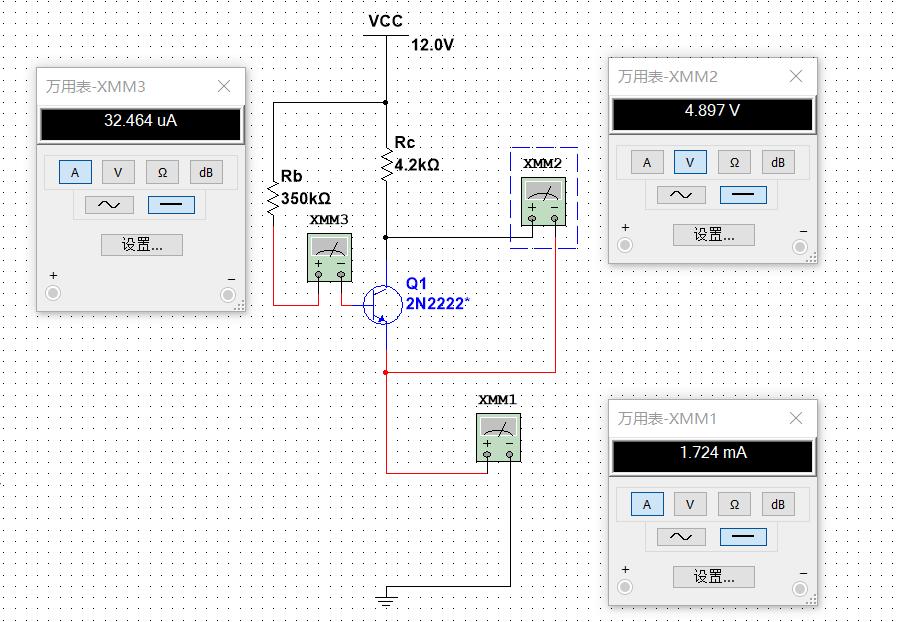
\includegraphics[width=8cm]{img/a.png}
  \caption{共射级放大电路静态工作点测量}
  \label{共射级放大电路静态工作点测量}
\end{figure}
由图可知,$I_{BQ}=32.464\mu A,I_{EQ}=1.724mA,V_{CEQ}=4.897V$

测量放大倍数的电路图如下:\par

\begin{figure}[h]
  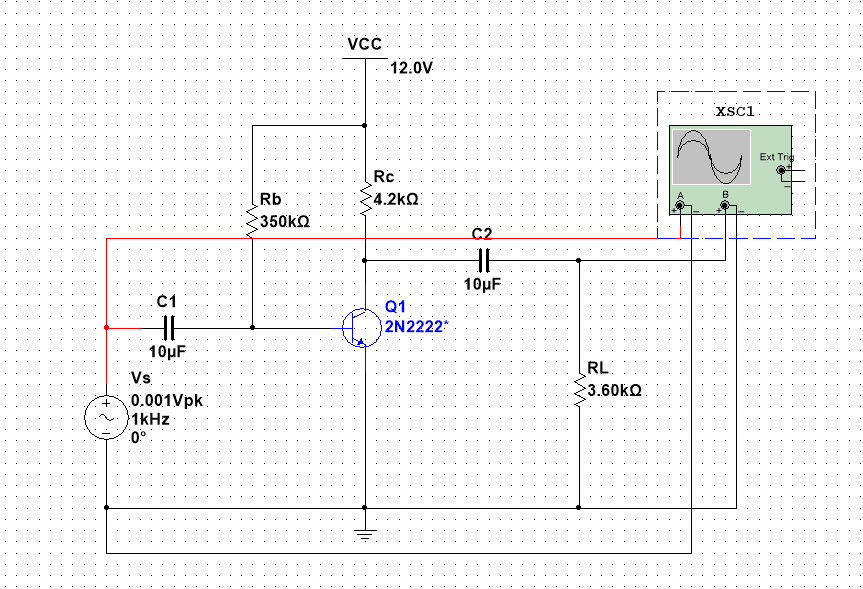
\includegraphics[width=8cm]{img/b.png}
  \caption{共射级放大电路放大倍数测量}
  \label{共射级放大电路放大倍数测量}
\end{figure}

示波器显示值如下:\par

\begin{figure}[h]
  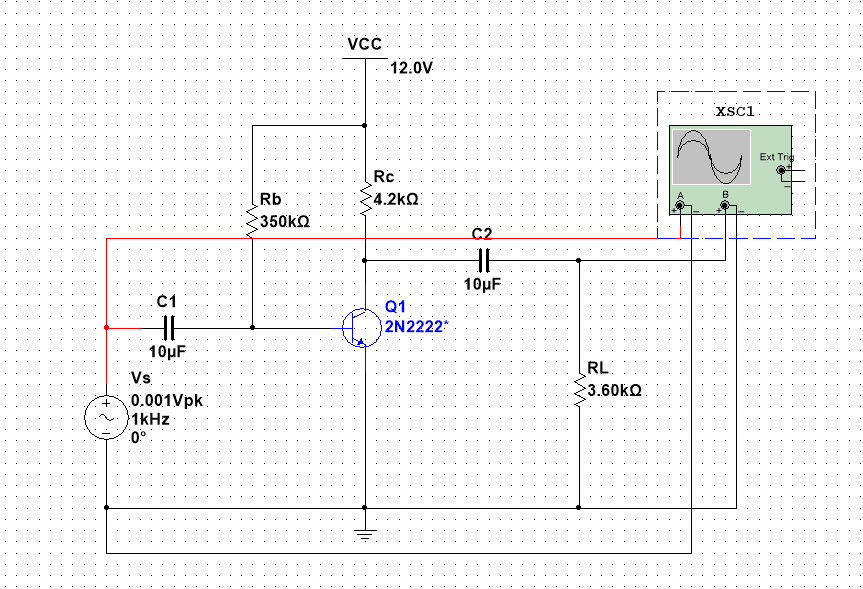
\includegraphics[width=8cm]{img/b.png}
  \caption{共射级放大电路放大倍数测量}
  \label{共射级放大电路放大倍数测量}
\end{figure}

由图可知$A_V = -103.318 / 0.989918 = -104.370261$ \par
在测量电路放大倍数的电路基础上,观察改变Rb大小出现的波形:\par

\paragraph{$V_s = 0.05V_{pk} , R_b = 15k\Omega$}图 4

\begin{figure}[h]
  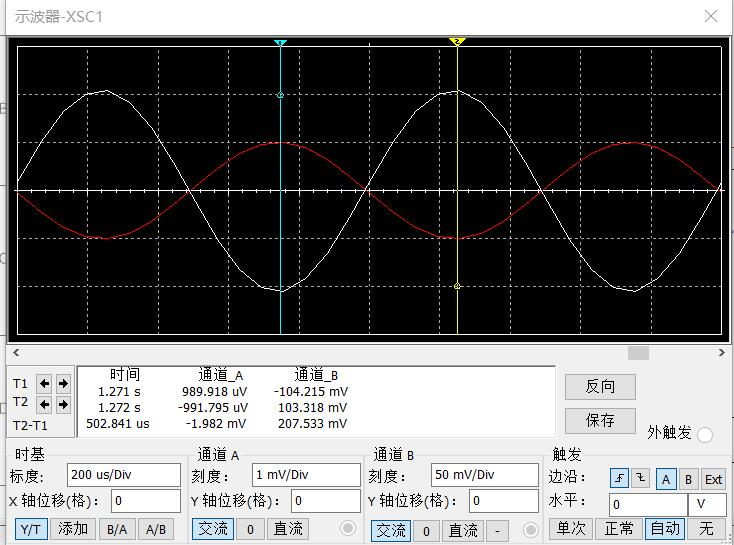
\includegraphics[width=8cm]{img/c.png}
  \caption{共射级放大电路的输出波形}
  \label{共射级放大电路的输出波形}
\end{figure}


\paragraph{$V_{s} = 0.05V_{pk} , R_b = 1000k\Omega$}图 5

\begin{figure}[h]
  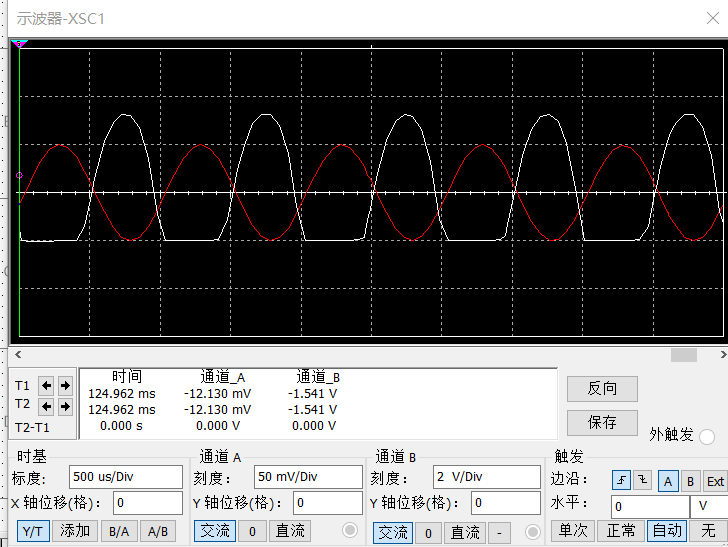
\includegraphics[width=8cm]{img/d.png}
  \caption{共射级放大电路的输出波形}
  \label{共射级放大电路的输出波形}
\end{figure}



\subsection{提高要求}
探究输入信号频率对输出电压的影响\par
在本题要求的电路基础上,不改变其他条件且电路不失真的情况下,
从1hz开始逐步增大输入电压的频率,观察输出电压波形的变化
%TODO: insert Picture
\begin{figure}[h]
  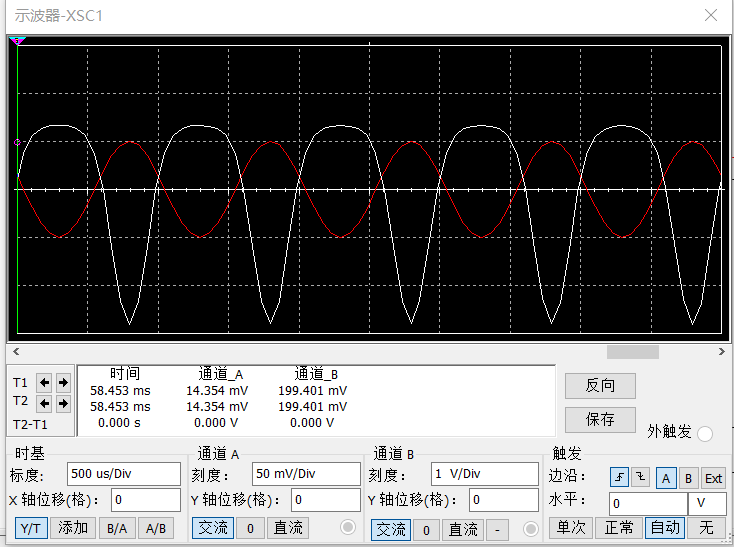
\includegraphics[width=8cm]{img/e.png}
  \caption{f = 1Hz Av=1.832/1.007=1.81926514}
%  \label{$f = 1Hz\    A_V=1.832/1.007=1.81926514$}
\end{figure}

\begin{figure}[h]
  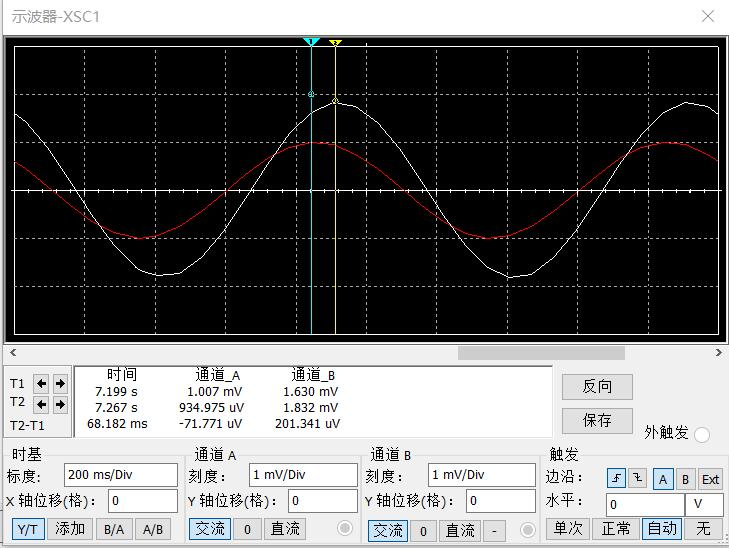
\includegraphics[width=8cm]{img/f.png}
  \caption{f = 100Hz Av = 101.158/0.986126 = 102.581212}
%  \label{$f = 1Hz\    A_V=1.832/1.007=1.81926514$}
\end{figure}

\begin{figure}[h]
  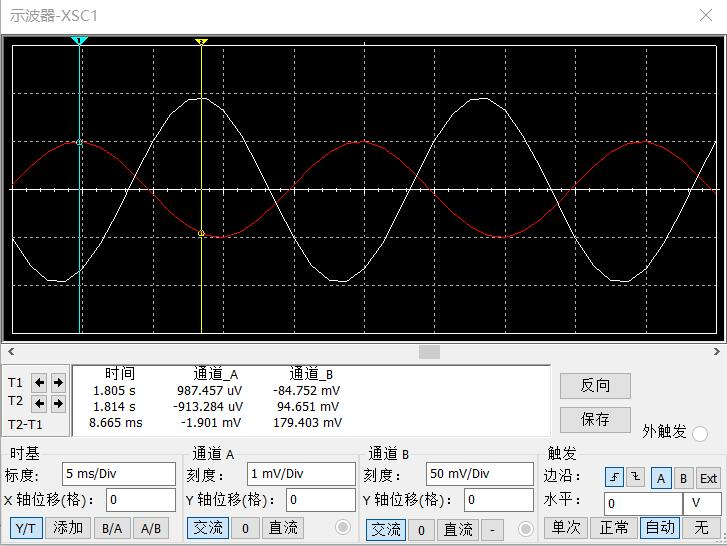
\includegraphics[width=8cm]{img/g.png}
  \caption{f = 100Hz Av = 101.158/0.986126 = 102.581212}
%  \label{$f = 1Hz\    A_V=1.832/1.007=1.81926514$}
\end{figure}

\begin{figure}[h]
  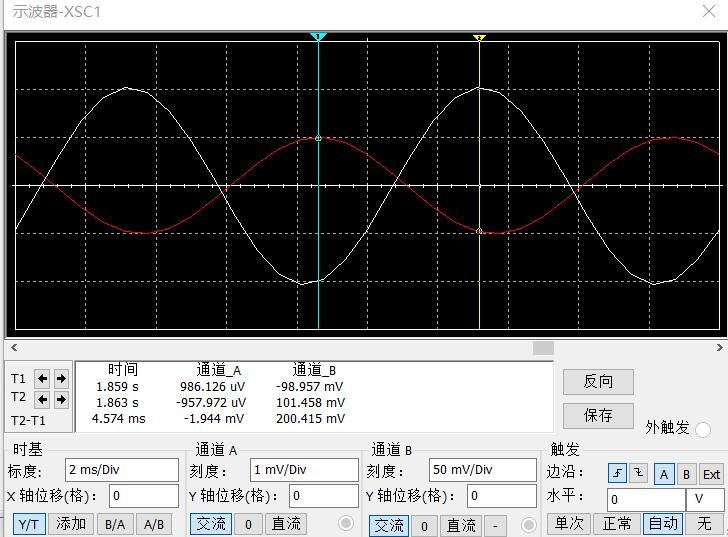
\includegraphics[width=8cm]{img/h.png}
  \caption{f = 10000Khz Av = 81.088/0.985738=82.2612094}
%  \label{$f = 1Hz\    A_V=1.832/1.007=1.81926514$}
\end{figure}

\begin{figure}[h]
  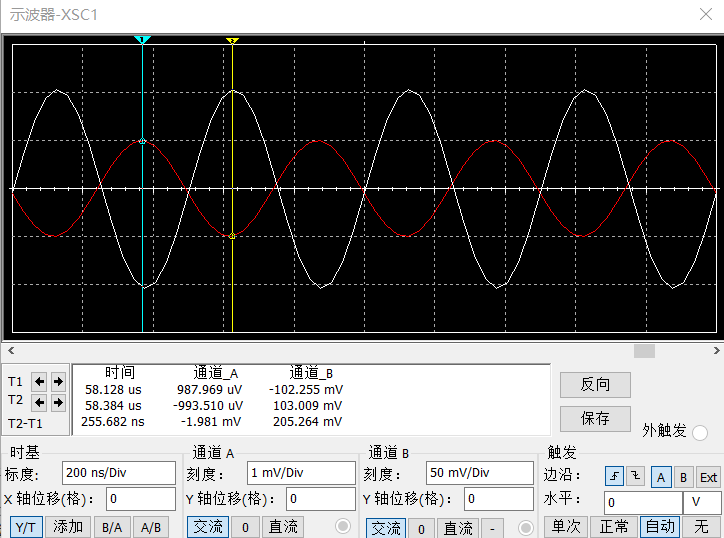
\includegraphics[width=8cm]{img/i.png}
  \caption{f = 20000Khz Av = 55.753/0.987840 = 56.4393019}
%  \label{$f = 1Hz\    A_V=1.832/1.007=1.81926514$}
\end{figure}

\begin{figure}[h]
  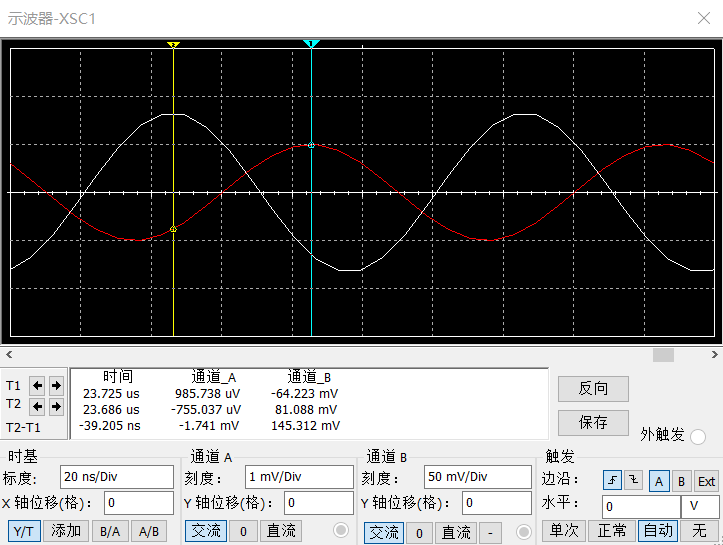
\includegraphics[width=8cm]{img/j.png}
  \caption{f = 50000Khz Av = 25.766/0.988617 = 26.0626714}
%  \label{$f = 1Hz\    A_V=1.832/1.007=1.81926514$}
\end{figure}



分析:\par
输入信号频率从1hz增大到100hz时,电压增益和相位差随频率增大而逐渐增大,
频率在100hz与2000khz之间时,电压增益和相位差几乎保持不变,
频率大于2000khz时,电压增益和相位差随频率增大而逐渐减小。

\subsection{结果分析及体会}
整个项目过程中,我们小组对问题的解决步骤都是比较明确的,
通过使用multisim软件进行了对共射极放大电路性质的测量及验证,
并在最后得出与预期差不多的结果,但在过程中还是存在一些问题。\par
首先由于是第一次使用multisim这个软件,所以在搭建电路上费了一些时间,
比如这个软件中电阻的图标与平时书上所看见的不同,但在搭建题目所要求的电路后,
测量的静态点值与理论值相差较大,经检查发现图中的三极管放大倍数与要求不符,
于是又花费了一些时间去查找修改放大参数的地方,
在此之后所有要求的参数以及要观察的波形都能以与预期相符的结果出现在示波器上。
通过这次实验,我们了解到在过程中遇到问题时,应当先分析问题出现的原因,
并在此基础之上发现整个实验的不足,这样可以对电路会有更好的理解,
并且,我们发现电路仿真软件可以让我们更方便地验证算出来的理论值是否正确,
也能更直观、更准确地观察到实验现象,
避免了在实际操作中可能出现的短路以及元器件烧坏等意外故障。

\section{思政综述}

由于物理学的重大突破,电子技术在20世纪取得了惊人的进步。
特别是50年来,微电子技术和其他高技术的飞速发展,
致使工业、农业、科技和国防等领域发生了令人瞩目的变革。
与此同时,电子技术也正改变着人们的日常生活。
基于此,作为电子技术基础研究课程的《模拟电子技术基础》应运而生。\cite{wang2009}
\par

《模拟电子技术基础》是通信工程的一门专业基础课,通过本课程的学习,
使学生掌握半导体基本器件的原理、特性及其应用,
了解和掌握常用模拟集成器件的外特性及其应用,
掌握基本电路单元的组成、工作原理及其重要性能指标的估算,
具有一定的读图能力和初步设计电路的能力,
具有一定的动手实践能力和解决问题的能力,为后续课程的学习打下良好的基础。\cite{li2009}
\par

《模拟电子技术基础》是继电路课程后,电气类、
自控类和电子类等专业学生在电子技术方面入门性质的技术基础课,
是电子技术基础的一个部分,其目的和任务是让学生获得模拟电路的基本知识,
为以后深入学习电子技术某些领域中的内容打下基础。
通过《模拟电子技术基础》课程的学习,使学生获得模拟电路的基本理论、
基本知识和基本技能,培养学生分析问题和解决问题的能力,
为模拟电子技术在专业中的应用打好基础。模电的前续课程是电路,
模电中应用了许多电路课程中的基本概念与方法,
例如迭加原理、戴维南定理、二端口网络、正弦交流电路的求解等,
应注意两门课在时间上的配合。模电的后续课程是数电、
EDA与电子技术课程设计、微机原理及其应用、电力电子、
检测与变换及各专业课程设计等,
模电课程中的半导体基本知识、
放大电路理论和各种集成电路知识将为这些后续课程的学习打下必要基础。\cite{huang2010}
\par

《模拟电子技术基础》是一门理论课程,
只有熟练的掌握相关电路规则与元器件的原理才能够尝试相关的实验,
并进行电路的设计。\par

笔者认为《模拟电子技术基础》是一门较为有趣的学科,
学习这门课程需要有高等数学、大学物理和电路基础等课程的基础。
就理论课而言,综合高数的微积分知识与大学物理中电路的基本关系,
再加上电路基础的一些电路规则与模电的相关定义规则来求解问题,
每验证出一个公式或推导出一个练习题都会有不小的成就感,
并且在熟练掌握了模电只是后,可以尝试设计简单的电路,
这也是不小的收获。从长远来看,模电作为理论课中承上启下的课程,
有助于我们深入学习相关的专业课程,并从事相关的设计工作,
更重要的是该课程可以教会我们一种全新的思考问题与解决问题的方式与方法,
让我们更有逻辑性,这对于我们以后的人生都是很非常重要的。\cite{zhou2013}
\par


% TODO: fix “笔者” -> "我们"
笔者认为《模拟电子技术基础》是一门较为有趣的学科,
学习这门课程需要有高等数学、大学物理和电路基础等课程的基础。
就理论课而言,综合高数的微积分知识与大学物理中电路的基本关系,
再加上电路基础的一些电路规则与模电的相关定义规则来求解问题,
每验证出一个公式或推导出一个练习题都会有不小的成就感,
并且在熟练掌握了模电只是后,可以尝试设计简单的电路,
这也是不小的收获。从长远来看,模电作为理论课中承上启下的课程,
有助于我们深入学习相关的专业课程,并从事相关的设计工作,
更重要的是该课程可以教会我们一种全新的思考问题与解决问题的方式与方法,
让我们更有逻辑性,这对于我们以后的人生都是很非常重要的。\cite{hu2013}
\par


电子信息技术水平是评判一个国家综合发展的关键准则,
对于一个国家而言,要想在激烈的国际竞争中占据有为有利的优势地位,
就必须在科学技术上有所创新与进步。电子信息技术为国家发展创造了全新的机遇,
在当前全球经济竞争的形势下,电子信息技术表现出极大的发展必然性。
在电子信息技术发展的过程中,衍生出一种全新的技术类别,我们称之为电子数据交换。
这技术最大的创新在于,完全扭转了之前需要人工参与的模式,
能够借助计算机,自动实现信息传送及数据资料的互换,实现了信息技术的智能化。
这一技术在实际工作中的运用打破了之前的生产模式,
为生产效率的提高创造了更为坚实的技术保障。并且,随着社会发展的需求,
这一技术在未来必定会运用到越来越多的行业范围内。从这里我们能够清楚的看出,
电子信息技术在我国经济建设及社会发展的过程中发挥着不可或缺的关键功能。
因此,不管是处于生产力水平的提升或者是经济实力的增强,
发展电子信息技术都具有一定的必然性。\par

电子信息技术的发展在现代社会中的发展具有极大的必然性,
是科学技术进步前行过程中必然产物,
在未来的发展中电子信息技术的发展必须建立在满足社会需求的基础上,
充分发挥自身的技术优势,努力实现自身发展与其他行业的彼此融合。
这样一来,电子信息技术的运用领域就能够得到进一步的扩宽,
同时,更为重要的是,能够有效推动社会各行业生产活动的高效开展。
就当前国际经济发展形势而言,一个国家发展与其电子信息技术发展水平有必然的关联,
这使得电子信息技术已经成为制约国家发展与进步的关键性影响因素,
所以电子信息技术在我国的发展体现出关键性的现实性意义。\par

电子信息技术的发展在现代社会中的发展具有极大的必然性,
是科学技术进步前行过程中必然产物,
在未来的发展中电子信息技术的发展必须建立在满足社会需求的基础上,
充分发挥自身的技术优势,努力实现自身发展与其他行业的彼此融合。
这样一来,电子信息技术的运用领域就能够得到进一步的扩宽,同时,更为重要的是,
能够有效推动社会各行业生产活动的高效开展。就当前国际经济发展形势而言,
一个国家发展与其电子信息技术发展水平有必然的关联,
这使得电子信息技术已经成为制约国家发展与进步的关键性影响因素,
所以电子信息技术在我国的发展体现出关键性的现实性意义。\par


在我国电子信息产业发展的过程中,环境资源的短缺紧缺,
也是一个不可忽略的重要因素。
这一问题最为明显的体现为当前市场上存在电子信息产品质量参差不齐,
尤其是对于软件研发领域,这一现象更为严重。
不仅如此,电子信息知识的产权维护问题也存在一定的缺陷,侵权现象屡禁不止,
有时候还会存在很多企业发生盗版走私、出售的行为活动。
如此一来,对于我国电子信息产业的规范化发展就形成了很大的限制性作用,
最终造成我国电子信息产业发展水平提升效率的降低。\par

除了人才资源及环境问题的限制,我国电子信息产业还面临着一个关键问题,
就是产业结构优化程度过低。随着社会发展及科学技术水平的进步,
这一问题正日益凸显出来。在过去几年的发展中,
我国的电子信息技术水平得到了极大的提升,取得了较为可观的成绩,
不过不可忽视的一个问题是,
与世界先进国家间的距离依然较大尤其是先进产品的研发与创新,
导致这一现象的原因主要是电子信息产业结构优化程度较低。
因此,对于我国电子信息产业而言,要想获取更为突出的发展效果,
就必须针对当前的产业结构加以完善与优化,
这将是电子信息产业未来发展需要重点注意的问题。\cite{chen2014}
\par

总的来说,科学技术是第一生产力,
对于一个国家而言,要想在社会经济建设中获取更多的力量支撑,
就必须注重于自身科学技术水平的提升,
这是一个国家及社会进步的根本保障。
从当前的情况来看,电子信息技术较之前有了较大的进步与发展,
正逐渐的涉及到社会各个行业领域,给我们的生活方式带来极大的转变。
但是就因为其运用领域的宽阔性,不可避免的导致一些问题的发生。
因此,必须要从实际出发,针对这些问题做出分析,并采取可行的措施予以应对,
只有这样才可以确保我国电子信息技术水平的进一步提升。\par


\section{团队分工}

于宗玄,薛昊辰:\par
对题目一的电路进行仿真,验证用理论计算方法得出的结果,
并在此基础之上进行提高要求(输入电压频率和输出电压的关系), 
根据观察到的波形以及得到的结果进行分析,最后进行总结。

胡潇丹,麻珂珂:\par
结合《模拟电技术基础》这门课程的学习,在利弊以及对未来的展望方面进行综述。

高浚哲:\par
对整个实验报告进行排版,并进行设计感想与致谢。


\section{时间进度}

2019年12月13日:确定项目并明确小组各个成员的分工\par
2019年12月14日:各个成员按照安排进行工作\par
2019年12月15日:汇总各个成员的结果,报告完成\par

\section{设计感想}
设计感想 TODO


\section{致谢}
感谢老师在本学期对我们的教导 TODO

%\thanks{感谢老师在本学期对我们的教导}
%\begin{figure}[h]
%	
\includegraphics[width=8cm]{school.jpg}
%	\caption{school} 
%	\label{school}
%\end{figure}


\begin{figure}[h]
  
\includegraphics[width=8cm]{img/nana.png}
  \caption{Nana Kaguya}
  \label{Nana Kaguya}
\end{figure}


\subsection{小节}
可以导入代码
%需要引用第三方库
%\begin{python}
%import numpy as np
%a = np.random.randn((5,5))
%\end{python}



\subsubsection{小小节}

\begin{equation}
  E= MC^2
\end{equation}


\begin{equation}
max(0,x)=\left\{
\begin{aligned}
0, \quad x \leq 0 & \\
1, \quad x > 0  &
\end{aligned}
\right.
\end{equation}

参考文献的引用:
\cite{yearbook2005china}



\bibliographystyle{IEEEtran} 
\bibliography{ref}   



%\end{CJK}
\end{document}
